\section{Overview} 
\label{sec:overview}

\begin{figure}[H]
    \centering



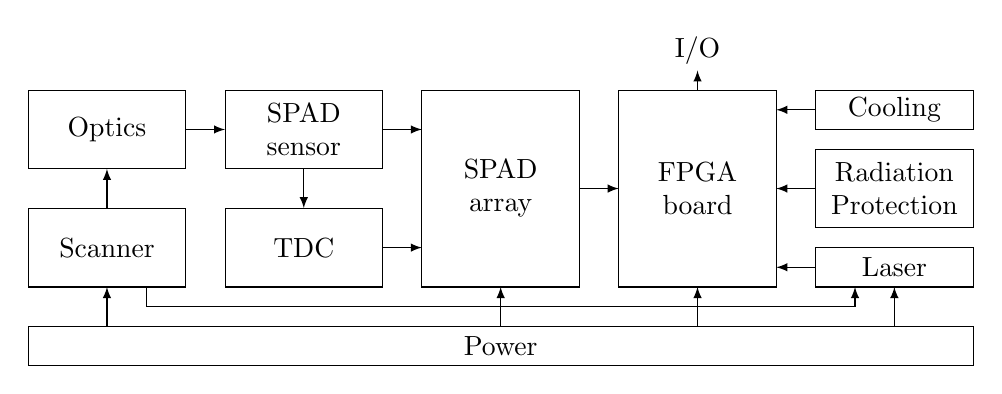
\begin{tikzpicture}[scale=.5]

\draw  (13,2) rectangle (17,1) node[pos=.5, align=center]{Cooling};
\draw  (13,0.5) rectangle (17,-1.5) node[pos=.5, align=center]{Radiation\\Protection};
\draw  (-7,-4) rectangle (17,-5) node[pos=.5, align=center]{Power};
\draw  (13,-2) rectangle (17,-3) node[pos=.5, align=center]{Laser};
\draw  (8,2) rectangle (12,-3) node[pos=.5, align=center]{FPGA\\board};
\draw  (3,2) rectangle (7,-3) node[pos=.5, align=center]{SPAD\\array};
\draw  (-2,2) rectangle (2,0) node[pos=.5, align=center]{SPAD\\sensor};
\draw  (-7,2) rectangle (-3,0) node[pos=.5, align=center]{Optics};
\draw  (-7,-1) rectangle (-3,-3) node[pos=.5, align=center]{Scanner};
\draw  (-2,-1) rectangle (2,-3) node[pos=.5, align=center]{TDC};

\draw [>=latex, ->](0,0) -- (0,-1);
\draw [>=latex, ->](2,-2) -- (3,-2);
\draw [>=latex, ->](13,1.5) -- (12,1.5);
\draw [>=latex, ->](7,-.5) -- (8,-.5);
\draw [>=latex, ->](2,1) -- (3,1);
\draw [>=latex, ->](13,-2.5) -- (12,-2.5);
\draw [>=latex, ->](10,2) -- (10,2.5);
\draw [>=latex, ->](-3,1) -- (-2,1);
\draw [>=latex, ->](13,-.5) -- (12,-.5);
\draw [>=latex, ->](5,-4) -- (5,-3);
\draw [>=latex, ->](10,-4) -- (10,-3);
\draw [>=latex, ->](15,-4) -- (15,-3);
\draw [>=latex, ->](-5,-1) -- (-5,0);
\node at (10,3) {I/O};

\draw [>=latex, ->](-5,-4) -- (-5,-3);
\draw [>=latex, ->](-4,-3) -- (-4,-3.5) -- (14,-3.5) -- (14,-3);

\end{tikzpicture}




    \caption{Schematic overview}
    \label{tkz:schematic_overview}
\end{figure}

\section{SPAD sensor} 
\label{sec:spad_sensor}
The SPAD Sensor generates a pulse when a photon is detected. It is connected to a TDC, and is used to construct a SPAD grid.

\subsection{requirements} 
\label{ssec:sensor_req}

\begin{table}[H]
    \begin{tabular}{l|l|l}
    ~                                  & Threshold & Goal \\ \hline
    Max Acquisition Slant Range        & 5 km      & 8 km \\
    Min Operational Range              & 5 m       & 1 m  \\
    Range Accuracy                     & 10 cm     & 5 cm \\
    Photon Detection Probability (PDP) & ?         & ?    \\
    Dead-time                          & ?         & ?    \\
    Dark count rate (DCR)              & ?         & ?    \\
    \end{tabular}
\end{table}

The most important requirement of the SPAD is the range accuracy of 5-10 cm. 

\begin{align*}
	\frac{5\cdot10^-2}{3\cdot10^8} &= 167\, ps 
\end{align*}

Therefore the jitter on the time between the arrival of a photon and the transmission of a pulse must be as small as possible.

\subsection{Possibilities} 
\label{ssec:sensor_pos}
To be continued

\subsection{Choice} 
\label{ssec:sensor_choice}
Basically we are going for CMOS Si SPAD's.


\section{TDC} 
\label{sec:tdc}
The Time intrerval to Digital Converted (TDC) is connected to a (or several) SPAD sensor. The TDC has to convert the difference in time between two pulses into a digital representation. It is used together with the SPAS sensors to build a SPAD grid.

\subsection{Requirements} 
\label{ssec:tdc_req}

\begin{table}[H]
    \begin{tabular}{l|l|l}
    ~                    & Threshold & Goal   \\ \hline
    accuracy             & 50 ps?    & 30 ps? \\
    jitter               & 30 ps?    & 10 ps? \\
    area per SPAD sensor & ?         & ?      \\
    power usage          & ?         & ?      \\
    \end{tabular}
\end{table}

\subsection{Possibilities} 
\label{ssec:tdc_pos}
There are a lot of possibilities here. But I don't know what technique they use to save on the amount of TDC's.

\subsection{Choice} 
\label{ssec:tdc_choice}


\section{SPAD grid} 
\label{sec:spad_grid}
The grid is the structure that implements the SPAD sensors and TDC's into a grid to measure 

\subsection{Requirements} 
\label{ssec:grid_req}

\begin{table}[H]
    \begin{tabular}{l|l|l}
    ~                                    & Threshold         & Goal              \\ \hline
    Update rate                          & 0.1 Hz            & 1 Hz              \\
    Ground Sample Distance               & 10 cm             & 5 cm              \\
    Ground Area Coverage at max altitude & 100 m times 100 m & 125 m times 125 m \\
    Time for 3D map creation             & 1 s               & 1 s               \\
    \end{tabular}
\end{table}

\subsection{Possibilities} 
\label{ssec:grid_pos}

\subsection{Choice} 
\label{ssec:grid_choice}
The unproposed master thesis board.

\section{FPGA board} 
\label{sec:fpga_board}

\subsection{Requirements} 
\label{ssec:grid_req}

\begin{table}[H]
    \begin{tabular}{l|l|l}
    ~                                    & Threshold         & Goal              \\ \hline
    Update rate                          & 0.1 Hz            & 1 Hz              \\
    Ground Sample Distance               & 10 cm             & 5 cm              \\
    Ground Area Coverage at max altitude & 100 m times 100 m & 125 m times 125 m \\
    Time for 3D map creation             & 1 s               & 1 s               \\
    \end{tabular}
\end{table}

Note that the relevant requirements are similar to the SPAD grid, because the SPAD grid has to generate the data, and the FPGA has to process it. 

\subsection{Possibilities} 
\label{ssec:grid_pos}

\subsection{Choice} 
\label{ssec:grid_choice}
The FPGA accompanying the unproposed master thesis board.

\section{Radiation protection} 
\label{sec:radiation_protection}

Because we cannot change the FPGA board to be more resilient against radiation. It  ight be necessary to protect the board with external components. 
\subsection{Requirements} 
\label{ssec:grid_req}

The FPGA has to survive a certain amounty of Cobalt-64 and proton radiation.

\subsection{Possibilities} 
\label{ssec:grid_pos}
The possibilities vary between different kinds of materials, different thickness, and positions. The possibility of no protection is also present.\\
\\


\subsection{Choice} 
\label{ssec:grid_choice}
The unproposed master thesis board.

\section{Laser} 
\label{sec:laser}
